\section{Motivação}

\begin{frame}[fragile]{Paradigmas de Programação}

    \begin{center}
        {\huge O que é \underline{paradigma}?}
    \end{center}

\end{frame}

\begin{frame}[fragile]{Paradigmas de Programação}

    \begin{center}
        {\huge O que é \underline{programação}?}
    \end{center}

\end{frame}

\begin{frame}[fragile]{Termos associados aos paradigmas de programação}

    \begin{figure}
        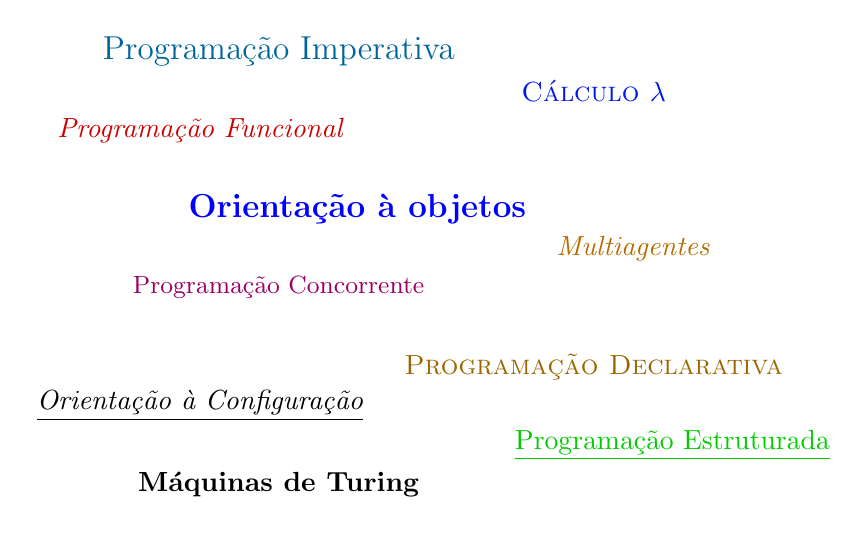
\begin{tikzpicture}
            \node[blue] at (-1, 1) { \bf \large Orientação à objetos };
            \node[red!80!black] at (-3, 2) { \it Programação Funcional };
            \node[green!80!black] at (3, -2) { \underline{Programação Estruturada} };
            \node[blue!60!green] at (-2, 3) { \large Programação Imperativa };
            \node[red!60!green] at (2, -1) { \sc Programação Declarativa };
            \node[red!60!blue] at (-2, 0) { \small Programação Concorrente };
            \node[color={rgb:red,4;green,2;yellow,1}] at (2.5, 0.5) { \it Multiagentes};
            \node[blue!90!green] at (2, 2.5) { \bf \sc Cálculo $\lambda$};
            \node[black] at (-2, -2.5) { \bf Máquinas de Turing };
            \node[black] at (-3, -1.5) { \it \underline{Orientação à Configuração} };
        \end{tikzpicture}
    \end{figure}

\end{frame}

\begin{frame}[fragile]{Benefícios do estudo dos paradigmas de programação}

    \begin{itemize}
        \item Aumento da capacidade de expressar ideias
        \item Escolhas bem fundamentadas das linguagens de programação a serem utilizadas em um 
            projeto
        \item Melhora na capacidade de aprendizado de novas linguagens
        \item Uso mais eficaz das linguagens já conhecidas
        \item Maior entendimento das diferentes implementações de um mesmo conceito
        \item Visão mais ampla da computação como um todo
    \end{itemize}

\end{frame}
